\section{What is Aging?}

\subsection{Definition and Hallmarks}

\begin{frame}[c]{Aging}
    \large

    \begin{block}{Definition \cite{sen2016epigenetic}}
        Aging is characterized by progressive decline in tissue and organ
        function and increased risk of mortality.
    \end{block}
    \pause
    But how can we measure it?
\end{frame}


\begin{frame}[c]{Hallmarks of Aging}
    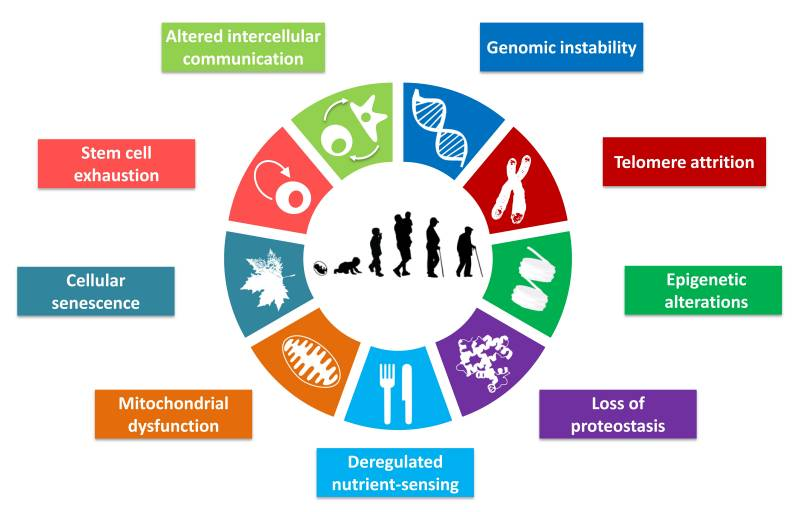
\includegraphics[width=\textwidth]{hallmarks_aging} \\
    Source: \cite{lopez2013hallmarks}
    % \begin{itemize}[<+(1)->]
    %     \item Genomic instability
    %     \item Telomere attrition
    %     \item Epigenetic alterations
    %     \item Loss of proteostasis
    %     \item Deregulated nutrient-sensing
    %     \item Mitochondrial dysfunction
    %     \item Cellular senescence
    %     \item Stem cell exhaustion
    %     \item Altered intercellular communication
    % \end{itemize}
\end{frame}

\subsection{Problematic: Many Unknowns}

\begin{frame}[c]{Problem: Many Theories}
    \large
    \begin{itemize}[<+(1)->]
        \item Everything is interlinked
        \item Very hard to distinguish cause and effect
        \item At least one Theory for every Hallmark
        \item Every prestigious lab has its own Theory
        \item A lot of speculation on all sides
        \item Unclear if we can already see the full picture
        \item More research is needed
    \end{itemize}
\end{frame}

\addtocounter{framenumber}{1}
\begin{frame}[standout]
    Disclaimer: Any misrepresentation or mistaken interpretation is due to my shortcomings
\end{frame}
